\documentclass[12pt]{article}

\usepackage[utf8x]{inputenc}
\usepackage[english]{babel}
\usepackage{subcaption}
\usepackage{amssymb,amsmath,amsthm,amsfonts}
\usepackage{calc}
\usepackage{graphicx}
\usepackage[shortlabels]{enumitem}
\usepackage{gensymb}
\usepackage{float}
\usepackage[numbers,sort&compress]{natbib}
\usepackage[colorlinks=true,
linkcolor=blue,
citecolor=blue,
urlcolor=blue]{hyperref}

\usepackage{url}
\usepackage[utf8x]{inputenc}
\usepackage{amsmath}
\usepackage{graphicx}
\graphicspath{{images/}}
\usepackage{parskip}
\usepackage{fancyhdr}
\usepackage{vmargin}
\usepackage{mathrsfs}
\usepackage[dvipsnames]{xcolor}
\usepackage{longtable}
\usepackage{multicol}
\usepackage{multirow}
\usepackage{booktabs}

%tikzpicture
\usepackage{tikz}
\usepackage{scalerel}
\usepackage{pict2e}
\usepackage{tkz-euclide}
\usetikzlibrary{calc}
\usetikzlibrary{patterns,arrows.meta}
\usetikzlibrary{shadows}
\usetikzlibrary{external}
\usepackage{listings}
\usepackage{xcolor}


\definecolor{lightgray}{rgb}{0.95,0.95,0.95}  % gris muy claro
% más oscuro:
% \definecolor{lightgray}{rgb}{0.9,0.9,0.9}
% aún más plomo:
% \definecolor{lightgray}{rgb}{0.85,0.85,0.85}

\lstset{
    language=C,
    basicstyle=\ttfamily\small,
    keywordstyle=\color{blue},
    commentstyle=\color{green!50!black},
    stringstyle=\color{red},
    numbers=left,
    numberstyle=\tiny,
    stepnumber=1,
    numbersep=5pt,
    frame=single,
    breaklines=true,
    tabsize=2
}
%pgfplots
\usepackage{pgfplots}
\pgfplotsset{compat=newest}
\usepgfplotslibrary{statistics}
\usepgfplotslibrary{fillbetween}

\setmarginsrb{3 cm}{2.5 cm}{3 cm}{2.5 cm}{1 cm}{1.5 cm}{1 cm}{1.5 cm}

\title{Parallelization of representative volume element (RVE) computations for a reduced order homogenization method for nonlinear materials}					% Titulo
\author{Matías I. Inostroza (mii2106)}					% Autor
\date{\today}						% Fecha


\makeatletter
\let\thetitle\@title
\let\theauthor\@author
\let\thedate\@date
\makeatother

\pagestyle{fancy}
\fancyhf{}
\rhead{\theauthor}
\lhead{Parallelization of RVE computations}
\cfoot{\thepage}

\begin{document}

%%%%%%%%%%%%%%%%%%%%%%%%%%%%%%%%%%%%%%%%%%%%%%%%%%%%%%%%%%%%%%%%%%%%%%%%%%%%%%%%%%%%%%%%%

\begin{titlepage}
	\centering
    \vspace*{0.0 cm}
    
\includegraphics[scale = 0.35]{Columbia_logo.png}\\[2.0 cm]	% Logo Universidad
    \textsc{\LARGE Columbia University}\\[2.0 cm]	% Nombre Universidad
	\textsc{\Large APMAE4302}\\[0.5 cm]				% Codigo Curso
	\textsc{\large Methods in computational science}\\[0.5 cm]		% Nombre Curso
	\rule{\linewidth}{0.2 mm} \\[0.4 cm]
	{ \huge \bfseries \thetitle}\\
	\rule{\linewidth}{0.2 mm} \\[1.5 cm]
	
	\begin{minipage}{0.4\textwidth}
		\begin{center} \large
			\emph{Author:}\\
			\theauthor\linebreak
			\end{center}
	\end{minipage}\\[2 cm]
	
	{May, 2026}\\[2 cm]
 
	\vfill
	
\end{titlepage}

%%%%%%%%%%%%%%%%%%%%%%%%%%%%%%%%%%%%%%%%%%%%%%%%%%%%%%%%%%%%%%%%%%%%%%%%%%%%%%%%%%%%%%%%%

\tableofcontents
\pagebreak

%%%%%%%%%%%%%%%%%%%%%%%%%%%%%%%%%%%%%%%%%%%%%%%%%%%%%%%%%%%%%%%%%%%%%%%%%%%%%%%%%%%%%%%%%
\section*{Abstract}


This project focuses on accelerating the offline stage of the Eigenstate Based Homogenization (EBH) method for nonlinear heterogeneous materials. In EBH, the reduced order response depends on influence tensors $E$ and $P$, which are computed by solving multiple independent RVE boundary value problems. The tensor $P$ is especially expensive because one problem must be solved for each partition and each independent strain mode. A task parallel DOLFINx implementation was developed using PETSc, MUMPS, and multi point constraints for periodic boundary conditions. Each MPI rank stores a complete copy of the RVE and solves a subset of the independent right hand side problems, while the stiffness matrix factorization is reused. The implementation was compared against an existing serial Fortran code and validated using the EBH online implementation provided by Junhe Cui. The results show that the proposed implementation consistently reduces the offline computation time while reproducing the reference EBH response.

\section{Introduction}
Many engineering materials, such as composites, polycrystals, and porous media, exhibit heterogeneous microstructures whose behavior strongly influences the macroscopic mechanical response. Performing a fully resolved finite element simulation that captures all microscopic features is typically computationally infeasible for real engineering structures, specially with those that exhibit nonlinear efects such as plasticity or damage. Multiscale homogenization provides an effective alternative by solving a local boundary value problem on a Representative Volume Element (RVE) whose averaged response defines the macroscopic constitutive law \cite{Fish2013,FishCuiEBH,Geers2010}.

\subsection{Linear first order homogenization}

A first order computational homogenization framework assumes that the macroscopic model is governed by the linear elasticity equations, where the effective stiffness tensor $L^c_{ijmn}$ replaces the heterogeneous microscopic constitutive law. To obtain this tensor, a microscale boundary value problem is solved on a representative volume element (RVE) $\Theta$ for each independent component of the macroscopic strain (3 normal components and 3 shear components in three dimensions).

Following the asymptotic homogenization framework presented by Fish \cite{Fish2013}, the fine scale displacement field is expanded into coarse scale and fluctuation contributions. The leading order displacement $u_i^{(0)}(\mathbf{x})$ represents the coarse scale displacement field, while the first order correction captures the periodic fluctuation induced by the microstructure. The first order displacement field is written as $u_k^{(1)}(\mathbf{x},\mathbf{y}) = H_k^{mn}(\mathbf{y})\,u^{(0)}_{m,x_n}(\mathbf{x})$, where $H_k^{mn}(\mathbf{y})$ is the first order displacement influence function associated with the macroscopic strain component $mn$, and $\mathbf{y}$ denotes the local coordinate inside the RVE.

Substitution of this decomposition into the microscopic equilibrium equation leads to the classical unit cell problem, subject to periodic boundary conditions over the unit cell.


\begin{eqnarray}
\left[ L_{ijkl} \left( I_{klmn} + H^{mn}_{k,y_l} \right) \right]_{,y_j} = 0 \qquad \text{in } \Theta \\ 
H_i^{mn}(\mathbf{y}) = H_i^{mn}(\mathbf{y}+\mathbf{l}) \qquad \text{on opposite boundaries of } \partial \Theta
\end{eqnarray}

Where $I_{klmn}$ is the fourth order symmetric identity tensor, and $\mathbf{l}$ is the length of the unit cell.
Together with a constraint to remove rigid body translations, such as a zero mean condition or vertex fixing.
Once the fluctuation field is obtained, the elastic strain influence tensor is defined as
\begin{equation}
\notag E_{kl}^{mn}(\mathbf{y}) = I_{klmn} + H_{k,y_l}^{mn}(\mathbf{y}) \rightarrow \text{ microscopic strain field } \rightarrow \varepsilon_{kl}^{f}(\mathbf{x},\mathbf{y}) = E_{kl}^{mn}(\mathbf{y}) \, \varepsilon_{mn}^{c}(\mathbf{x})
\end{equation}

Where $\varepsilon_{mn}^{c}(\mathbf{x})$ is the coarse strain. The corresponding stress influence function is therefore:

\begin{equation}
\Sigma_{ij}^{mn}(\mathbf{y}) = L_{ijkl}(\mathbf{y}) E_{kl}^{mn}(\mathbf{y})
\end{equation}

Finally, the homogenized constitutive tensor is obtained by volume averaging over the unit cell domain:

\begin{equation}
L^{c}_{ijmn} = \frac{1}{|\Theta|} \int_{\Theta}\Sigma_{ij}^{mn}(\mathbf{y}) \,d\Theta.
\end{equation}

Therefore, the unit cell problem consists of solving the RVE subjected to periodic boundary conditions and six independent unit macroscopic strain modes ($xx$, $yy$, $zz$, $xy$, $yz$, and $xz$). The resulting influence functions are then used to compute the effective constitutive tensor governing the macroscopic response.

\subsection{Reduced order homogenization: Eigenstate Based Homogenization (EBH)}
Although first order computational homogenization provides accurate effective constitutive properties, nonlinear multiscale simulations remain computationally expensive because many microscopic boundary value problems must be solved during the loading process. Reduced order homogenization methods alleviate this limitation by reducing the number of unknowns required to represent the microscale response while preserving the essential mechanical behavior of heterogeneous materials.

One such framework is the Eigenstate Based Homogenization (EBH) method proposed by Fish and Cui \cite{FishCuiEBH}. Instead of solving for all finite element degrees of freedom inside the Representative Volume Element (RVE), the microscale response is approximated using precomputed influence functions associated with macroscopic strains and partition level eigenstrains.

In EBH, the microscale displacement field is decomposed as

\begin{equation}
u_i(\mathbf{x},\mathbf{y}) = H_i^{kl}(\mathbf{y})\,\bar{\varepsilon}_{kl}(\mathbf{x}) + \int_{\Theta} h_i^{kl}(\mathbf{y},\tilde{\mathbf{y}}) \,
\mu_{kl}(\mathbf{x},\tilde{\mathbf{y}}) \,d\tilde{\Theta}
\end{equation}

where $H_i^{kl}$ are the displacement influence functions associated with the macroscopic strain field, while $h_i^{kl}$ are the transformation influence functions associated with the eigenstrain field $\mu_{kl}$. The microscale constitutive relation is

\begin{equation}
\sigma_{ij} = L_{ijkl} \left( \varepsilon_{kl}-\mu_{kl}\right)
\end{equation}

where $\mu_{kl}$ represents eigenstrains generated by nonlinear effects such as plasticity or damage.

To reduce the dimensionality of the problem, the eigenstrain field is approximated using partition functions,

\begin{equation}
\mu_{ij}(\mathbf{y}) =\sum_{A=1}^{M}N^A(\mathbf{y})\,\mu^A_{ij}
\end{equation}

where $M$ is the number of partitions and $\mu^A_{ij}$ are partition level eigenstates. In the limiting linear case, each material phase can be represented by a single partition, while nonlinear problems generally require a finer partition discretization to accurately capture localized inelastic behavior.

Using this approximation, the average strain in partition $B$ is written as

\begin{equation}
\varepsilon^{B}_{ij}=E^{Bkl}_{ij}\,\bar{\varepsilon}_{kl}+P^{BAkl}_{ij}\,\mu^A_{kl}
\end{equation}

where $E^{Bkl}_{ij}$ and $P^{BAkl}_{ij}$ are partition level influence tensors.

The tensor $E^{Bkl}_{ij}$ represents the strain response in partition $B$ due to a unit macroscopic strain and is computed as

\begin{equation}
E^{Bkl}_{ij}=\frac{1}{|\Theta^B|}\int_{\Theta^B}\left(H^{kl}_{i,y_j}+I_{ijkl}\right)\,d\Theta
\end{equation}

Similarly, $P^{BAkl}_{ij}$ represents the strain response in partition $B$ produced by a unit eigenstrain applied only in partition $A$ under periodic boundary conditions,

\begin{equation}
P^{BAkl}_{ij}=\frac{1}{|\Theta^B|}\int_{\Theta^B}\int_{\Theta}h^{kl}_{i,y_j}(\mathbf{y},\tilde{\mathbf{y}})\,N^A(\tilde{\mathbf{y}})\,d\tilde{\Theta}\,d\Theta
\end{equation}

Therefore, the computation of $P$ is analogous to the computation of the classical influence tensor $H$, but restricted to partition level eigenstrain excitations. For each partition, six unit deformation modes ($xx$, $yy$, $zz$, $xy$, $yz$, $xz$) must be solved independently.

The tensors $E$ and $P$ are computed during the offline stage through a sequence of independent elastic RVE problems. As the number of partitions increases, the number of required RVE solves grows significantly, leading to substantial computational cost. However, since these influence problems are fully independent, the EBH offline stage is naturally suitable for parallel computing. This project focuses on the parallelization of the partition level RVE computations required to assemble the influence tensor $P$, aiming to reduce the offline computational time and improve scalability for nonlinear multiscale simulations.

\section{Objectives}

\subsection{General objective}

The main objective of this project is to parallelize the computation of the EBH influence tensors $E$ and $P$ in order to reduce the offline computational cost associated with nonlinear multiscale simulations.

\subsection{Specific objectives}

\begin{itemize}
    \item Implement the EBH offline stage using the FEniCS/DOLFINx finite element framework with periodic boundary conditions for representative volume element (RVE) computations.

    \item Develop a task parallel strategy for the computation of the partition level influence tensors $E$ and $P$, exploiting the independence of the associated RVE problems.

    \item Compare the computational performance of the proposed FEniCS/DOLFINx implementation against an existing serial Fortran implementation of the EBH offline stage.

    \item Verify the correctness of the computed influence tensors by comparing the obtained results with the EBH online implementation provided by Junhe Cui.

    \item Analyze the scalability of the proposed parallelization approach as the number of RVE partitions increases.
\end{itemize}

\section{Methods}
\subsection{Representative volume element}
First, the RVE was generated using Gmsh, following the same general structure presented in the EBH paper \cite{FishCuiEBH}, consisting of a fiber embedded in a matrix. The geometric parameters are listed in Table~\ref{tab:rve_geometry}.

\begin{table}[h!]
\centering
\caption{RVE geometry.}
\begin{tabular}{cc}
\hline
Geometry & Value \\
\hline
Cube length & 1 \\
Fiber radius & 0.35 \\
Volume fraction $f$ & $\approx 40\%$ \\
\hline
\end{tabular}
\label{tab:rve_geometry}
\end{table}

The mesh consists of linear hexahedral elements arranged in a structured configuration, which allows the matrix phase to be divided into strip like partitions. It is important to highlight that only the matrix phase is partitioned. The front face contains 96 quadrilateral elements belonging to the matrix phase, allowing up to 96 matrix partitions. Table~\ref{tab:rve_mesh} summarizes the mesh discretization details.

\begin{table}[h!]
\centering
\caption{RVE mesh discretization.}
\begin{tabular}{cccc}
\hline
Element type & Gauss points per element & Number of nodes & Number of elements \\
\hline
Hexahedron & 8 & 1183 & 936 \\
\hline
\end{tabular}
\label{tab:rve_mesh}
\end{table}

Finally, the elastic parameters considered for the offline stage are listed in Table~\ref{tab:material_parameters}.

\begin{table}[h!]
\centering
\caption{Linear elastic material parameters.}
\begin{tabular}{ccc}
\hline
Material & Young's modulus $E$ [MPa] & Poisson's ratio $\nu$ \\
\hline
Matrix & 100 & 0.3 \\
Fiber & 10000 & 0.3 \\
\hline
\end{tabular}
\label{tab:material_parameters}
\end{table}

Figure \ref{fig:rve_mesh} shows the structured hexahedral mesh of the representative volume element (RVE) used in the EBH offline computations.

\begin{figure}[htbp]
    \centering
    \begin{subfigure}[t]{0.48\textwidth}
        \centering
        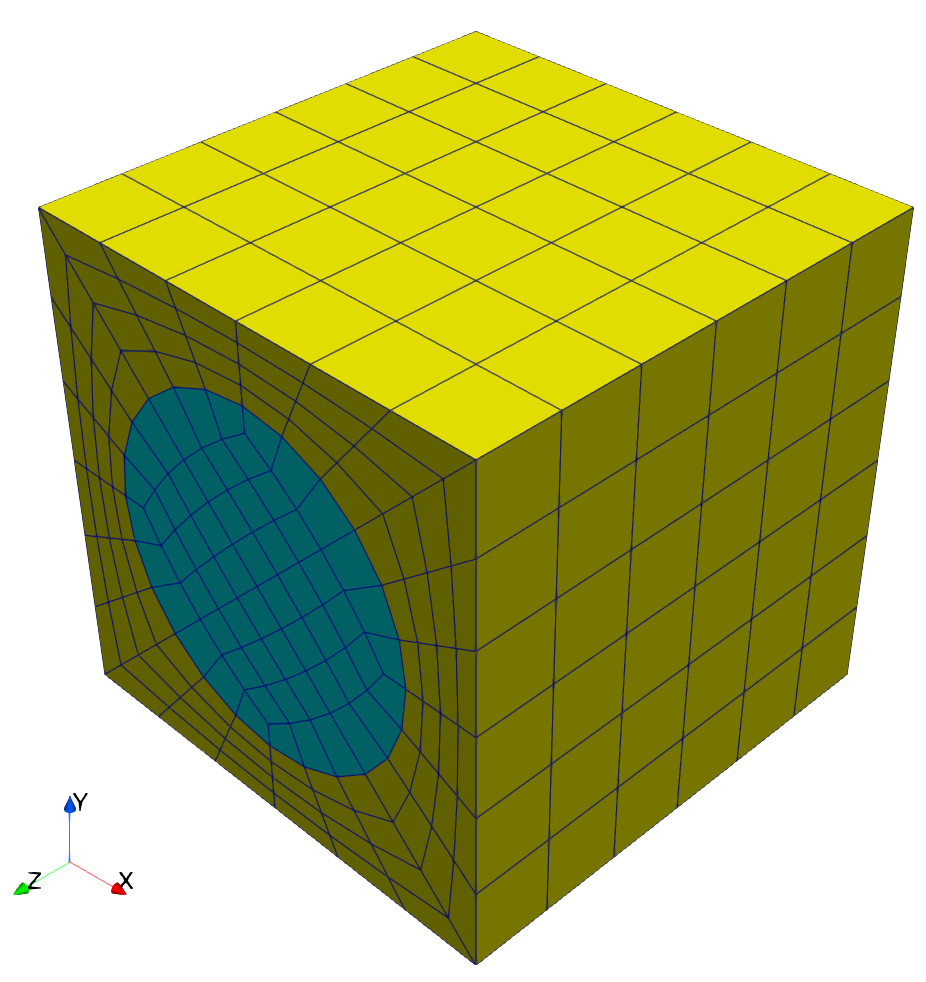
\includegraphics[width=5cm]{Figures/iso.png}
        \caption{Isometric view}
        \label{fig:rve_iso}
    \end{subfigure}\hfill
    \begin{subfigure}[t]{0.48\textwidth}
        \centering
        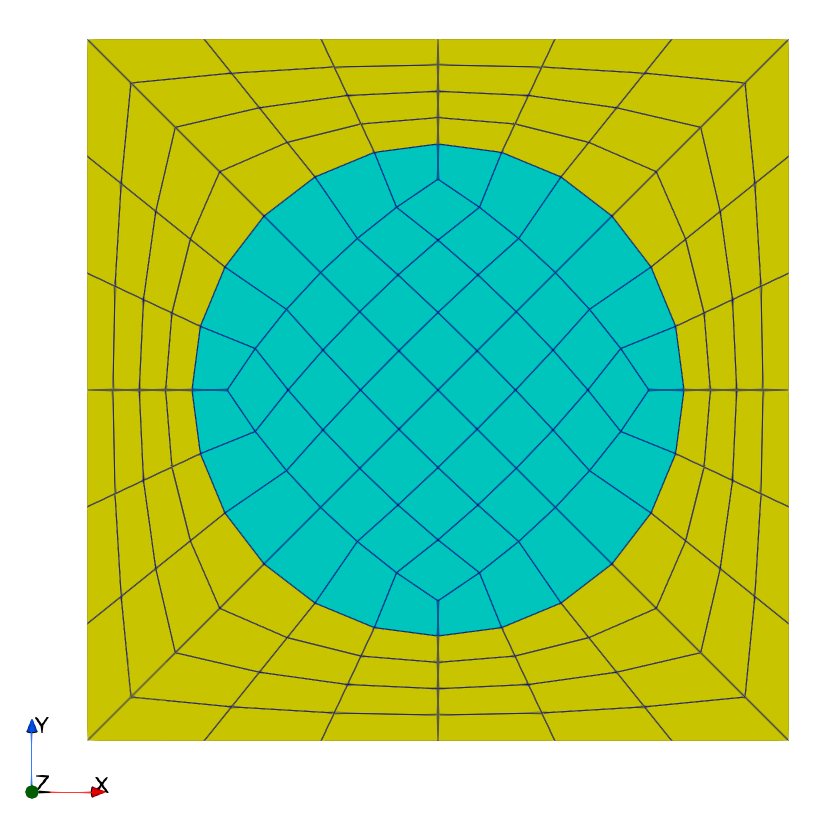
\includegraphics[width=5cm]{Figures/front.png}
        \caption{Front view}
        \label{fig:rve_front}
    \end{subfigure}
    \caption{RVE mesh.}
    \label{fig:rve_mesh}
\end{figure}

\subsection{Partitions}

In the EBH framework, the nonlinear internal variables are approximated at the partition level. Following the methodology proposed by Fish and Cui \cite{FishCuiEBH}, only the matrix phase is partitioned, while the fiber phase is treated as a single partition. This assumption is motivated by the fact that nonlinear effects are expected to evolve mainly inside the matrix material, whereas the fiber response remains predominantly elastic.

The matrix partitions are constructed from the structured discretization of the RVE mesh. Since the front face of the matrix contains 96 quadrilateral elements, the matrix can be divided into up to 96 independent partitions. Each partition represents a local eigenstrain region associated with the EBH reduced order approximation.


\begin{figure}[H]
    \centering

    % ---------------- Row 1 ----------------
    \begin{subfigure}[b]{0.25\textwidth}
        \centering
        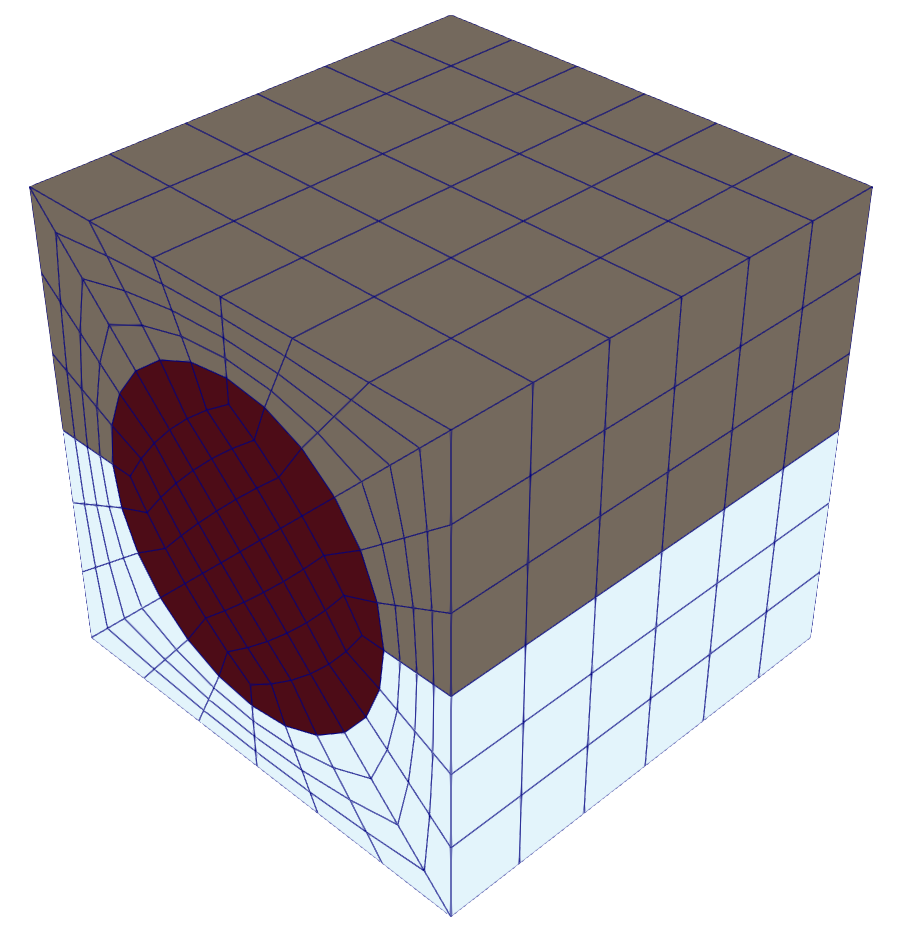
\includegraphics[width=\textwidth]{Figures/2.png}
        \caption{2 partitions}
    \end{subfigure}
    \hfill
    \begin{subfigure}[b]{0.25\textwidth}
        \centering
        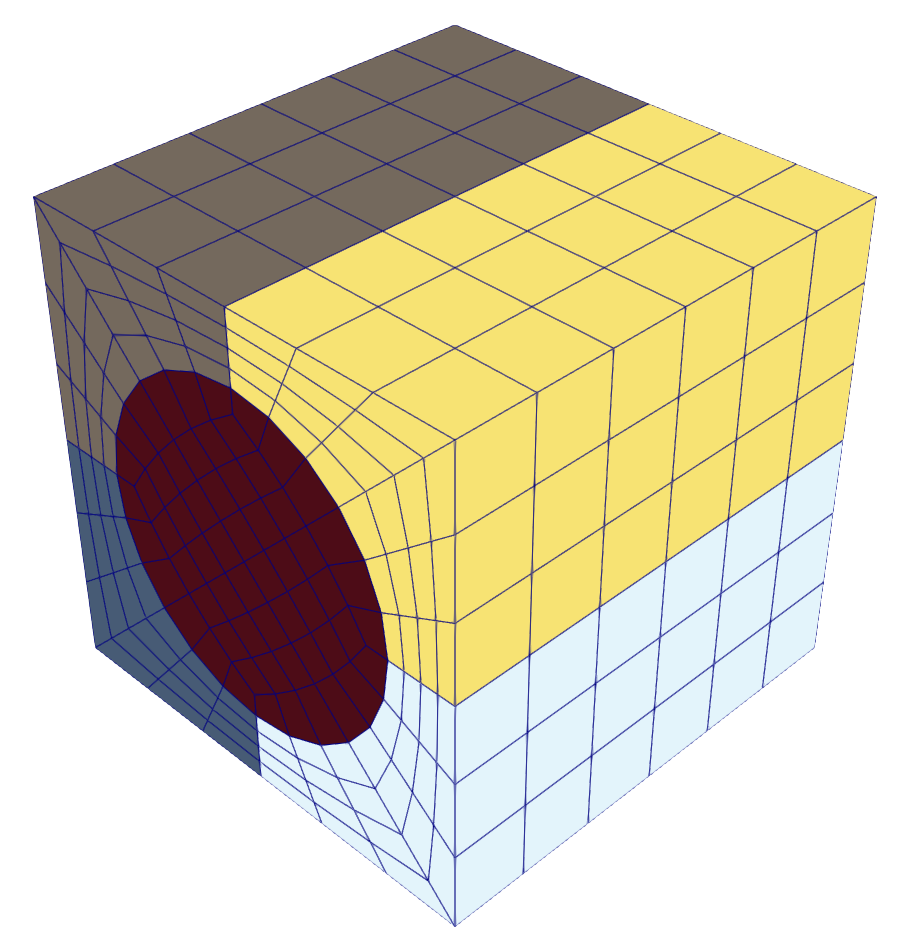
\includegraphics[width=\textwidth]{Figures/4.png}
        \caption{4 partitions}
    \end{subfigure}
    \hfill
    \begin{subfigure}[b]{0.25\textwidth}
        \centering
        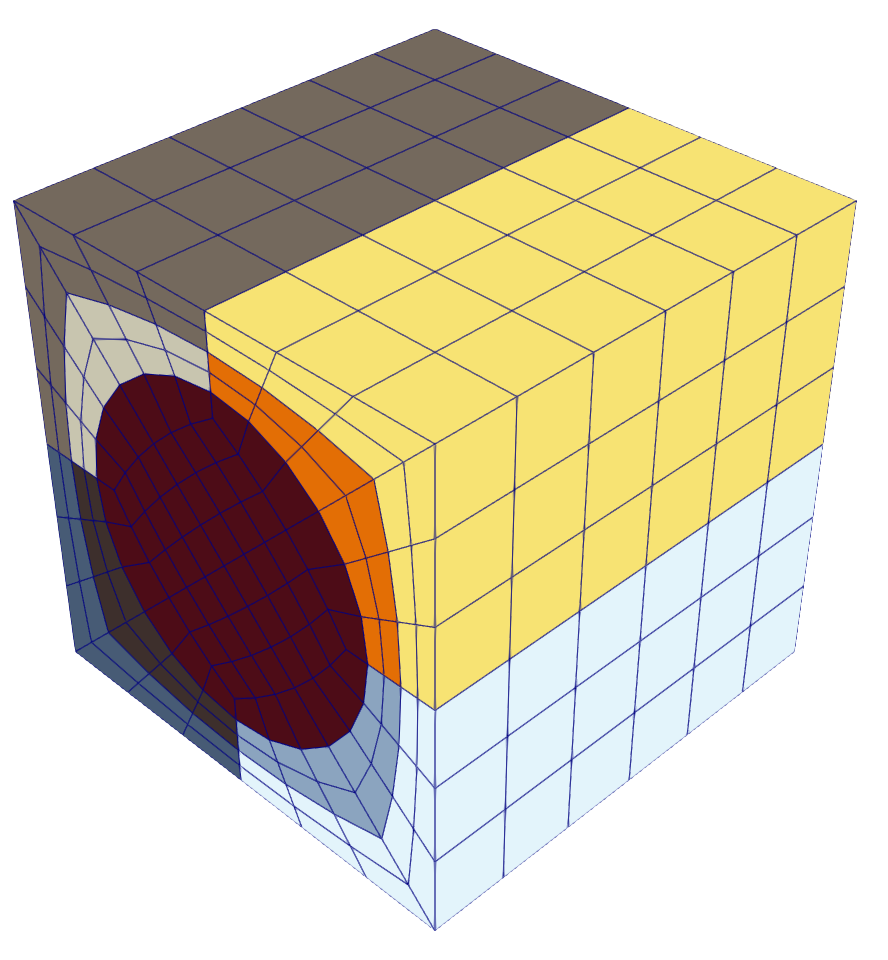
\includegraphics[width=\textwidth]{Figures/8.png}
        \caption{8 partitions}
    \end{subfigure}

    \vspace{0.5cm}

    % ---------------- Row 2 ----------------
    \begin{subfigure}[b]{0.25\textwidth}
        \centering
        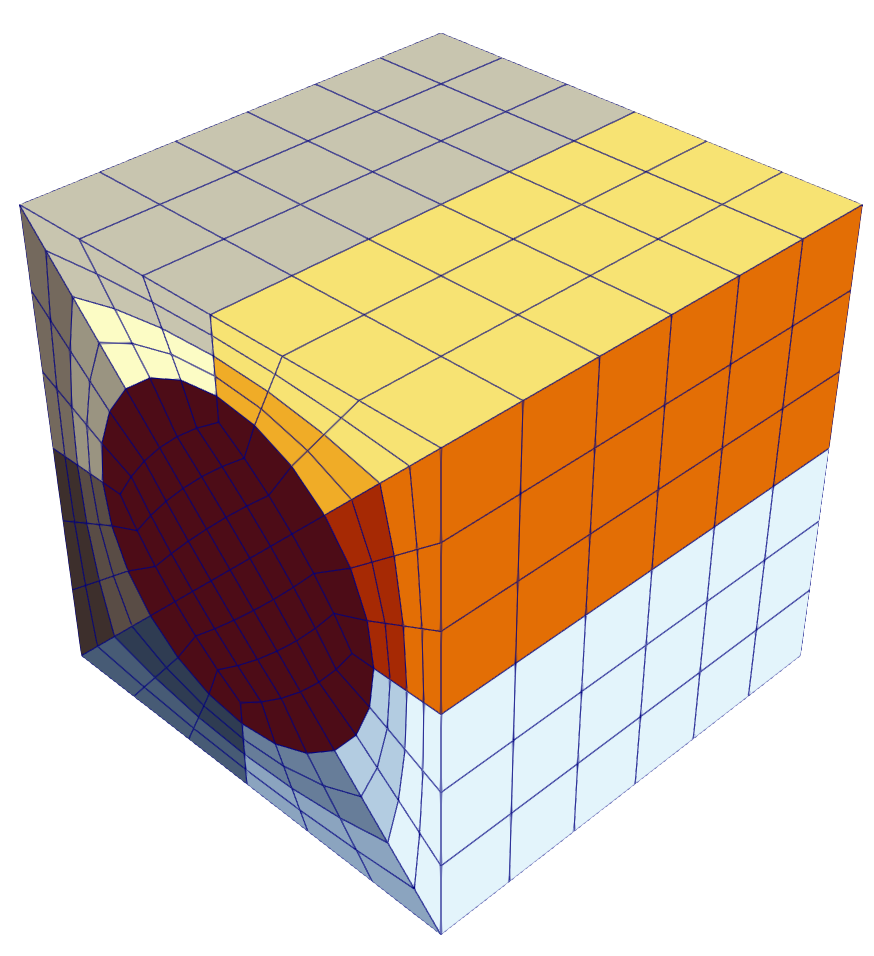
\includegraphics[width=\textwidth]{Figures/16.png}
        \caption{16 partitions}
    \end{subfigure}
    \hfill
    \begin{subfigure}[b]{0.25\textwidth}
        \centering
        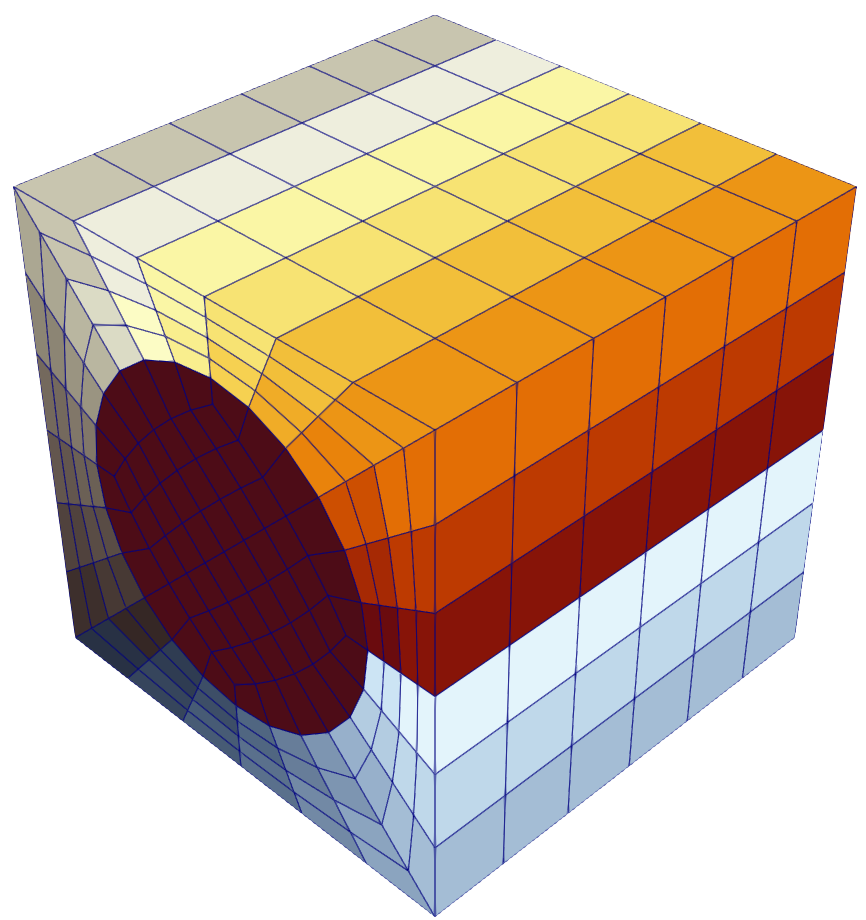
\includegraphics[width=\textwidth]{Figures/48.png}
        \caption{48 partitions}
    \end{subfigure}
    \hfill
    \begin{subfigure}[b]{0.25\textwidth}
        \centering
        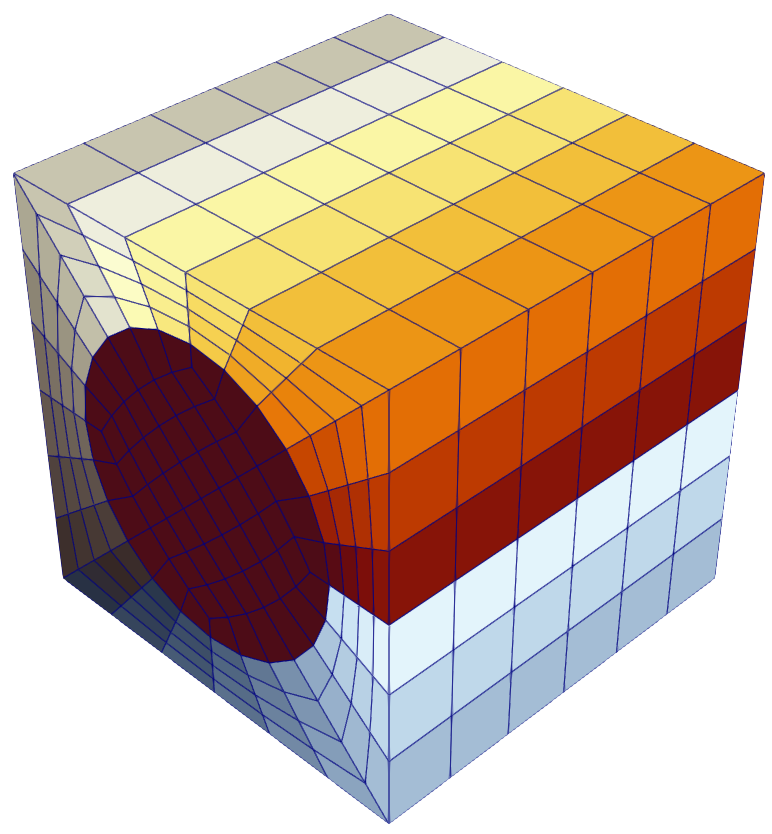
\includegraphics[width=\textwidth]{Figures/96.png}
        \caption{96 partitions}
    \end{subfigure}

    \caption{Radial-angular partitioning of the matrix phase for different numbers of partitions used in the EBH offline stage.}
    \label{fig:partitioning_levels}
\end{figure}

Figure~\ref{fig:partitioning_levels} shows the radial angular partitioning strategy adopted in this work for different numbers of matrix partitions. The colored regions indicate the individual matrix partitions used during the offline stage to compute the partition level influence tensor $P^{BAkl}_{ij}$. As the number of partitions increases, the reduced order model is able to capture more localized nonlinear behavior, at the expense of requiring a larger number of independent RVE solves.

\subsection{FEniCS code and parallelization}
The EBH offline stage was implemented using DOLFINx, PETSc, and \texttt{dolfinx\_mpc}. The objective of the code is to compute the influence tensors $E$ and $P$ associated with the reduced order homogenization formulation. The RVE mesh is imported from a Gmsh file, where the matrix and fiber phases are identified through physical tags. The displacement field is discretized using first order vector Lagrange elements, while material properties and partition indicator functions are represented using piecewise constant discontinuous functions.

Periodic boundary conditions are imposed using multi point constraints. Opposite faces, edges, and corners of the RVE are identified geometrically, and slave degrees of freedom are mapped to their corresponding master degrees of freedom. A small set of corner degrees of freedom is fixed to remove rigid body translations. This produces a constrained finite element system of the form \cite{FishBelytschko2007} $K u = f,$ where $K$ is the elastic stiffness matrix of the periodic RVE.

A key property of the EBH offline stage is that the stiffness matrix $K$ remains unchanged for all influence problems. Only the right hand side changes depending on the macroscopic strain mode or the partition level eigenstrain excitation. Therefore, the code assembles and factorizes the constrained stiffness matrix only once per MPI rank. This is done through a reusable PETSc linear solver, where the matrix is assembled with the MPC constraints and solved using a direct LU factorization with MUMPS. After this factorization, each influence problem only requires assembling a new right hand side and performing a back substitution:
\begin{equation}
u^{(q)} = K^{-1} f^{(q)}
\end{equation}

This avoids repeatedly assembling and factorizing the same stiffness matrix for every partition excitation.

The RVE domain is divided into one fiber partition and several matrix partitions. In the present implementation, the matrix is divided using a radial angular strategy. The angular coordinate separates the matrix into $N_\theta$ sectors around the fiber, while a normalized radial coordinate divides each sector into $N_r$ layers between the fiber boundary and the outer square boundary of the RVE. Thus, the total number of partitions is $N_{\mathrm{part}} = 1 + N_\theta N_r$, where the first partition corresponds to the fiber. For example, with $N_\theta=24$ and $N_r=4$, the model contains $N_{\mathrm{part}} = 1 + 24 \times 4 = 97$ partitions.

The computation of the tensor $E$ requires solving six independent problems, one for each macroscopic strain mode:
\begin{equation}
K H^{kl} = f_E^{kl},
\qquad kl = 1,\ldots,6.
\end{equation}
After each solution, the partition averaged strain is computed as
\begin{equation}
E^{Bkl}_{ij} = \frac{1}{|\Theta^B|}\int_{\Theta^B}\left(H^{kl}_{i,y_j}+I_{ijkl}\right) d\Theta 
\end{equation}

The computation of the tensor $P$ is more expensive. For every source partition $A$ and every strain mode $kl$, an independent RVE problem is solved:
\begin{equation}
K h^{Akl} = f_P^{Akl} ,\qquad A=1,\ldots,N_{\mathrm{part}}, \qquad kl=1,\ldots,6.
\end{equation}
The corresponding influence tensor is then obtained by averaging the resulting strain field over each target partition $B$ \cite{Fish2013}:
\begin{equation}
P^{BAkl}_{ij} = \frac{1}{|\Theta^B|} \int_{\Theta^B} h^{Akl}_{i,y_j}  d\Theta 
\end{equation}
Therefore, the number of independent $P$ solves is $N_P = 6N_{\mathrm{part}}$

For a case with 2 partitions (for example, fiber and matrix), the influence function $P^{BAkl}_{ij}$ takes the form of a matrix of size $12\times12$

\begin{equation}
\mathbf{P}
=
\begin{bmatrix}
\boxed{
\begin{matrix}
P^{11}_{xx,xx} & \cdots & P^{11}_{xx,xz} \\
\vdots & \ddots & \vdots \\
P^{11}_{xz,xx} & \cdots & P^{11}_{xz,xz}
\end{matrix}}
&
\boxed{
\begin{matrix}
P^{12}_{xx,xx} & \cdots & P^{12}_{xx,xz} \\
\vdots & \ddots & \vdots \\
P^{12}_{xz,xx} & \cdots & P^{12}_{xz,xz}
\end{matrix}}
\\[1.5em]
\boxed{
\begin{matrix}
P^{21}_{xx,xx} & \cdots & P^{21}_{xx,xz} \\
\vdots & \ddots & \vdots \\
P^{21}_{xz,xx} & \cdots & P^{21}_{xz,xz}
\end{matrix}}
&
\boxed{
\begin{matrix}
P^{22}_{xx,xx} & \cdots & P^{22}_{xx,xz} \\
\vdots & \ddots & \vdots \\
P^{22}_{xz,xx} & \cdots & P^{22}_{xz,xz}
\end{matrix}}
\end{bmatrix}
\end{equation}

This is a fully coupled matrix that describes how the strain response in one partition is influenced by an eigenstrain excitation applied to another partition.

For the case $N_{\mathrm{part}}=97$, this gives
\begin{equation}
N_P = 6 \times 97 = 582
\end{equation}
independent right hand side problems.

The parallelization strategy exploits this independence. Instead of decomposing the RVE mesh across MPI ranks, each MPI rank stores a complete copy of the RVE mesh and solves a subset of the independent right hand sides. This is implemented by assigning each task an integer index, $q = 6(A-1) + kl$ and distributing tasks according to
$q \bmod N_{\mathrm{rank}} = r$, where $r$ is the MPI rank. In this way, each rank solves approximately $\frac{6N_{\mathrm{part}}}{N_{\mathrm{rank}}}$ partition excitation problems.

This approach corresponds to task parallelism over independent right hand sides. It is particularly effective for the EBH offline stage because the RVE problems are independent, the stiffness matrix is reused, and communication is required only at the end of the computation. Each rank computes its local contribution to $P$, and the full tensor is assembled using an MPI reduction:
\begin{equation}
P = \sum_{r=0}^{N_{\mathrm{rank}}-1} P^{(r)}
\end{equation}
The same procedure is used for the six $E$ problems, although the computational benefit is smaller because only six macroscopic strain modes are involved.

The main advantage of this strategy is that it avoids the overhead of domain decomposition for relatively small RVE meshes while still distributing the dominant cost of the offline stage. Since the EBH offline computation involves many independent right hand sides, this task parallel implementation is well suited for shared memory or distributed memory high performance computing environments.
\section{Results}
\subsection{Fortran reference implementation}

The computational time of the proposed parallel DOLFINx implementation is compared against an existing Fortran implementation of the EBH offline stage. The Fortran code solves the same sequence of linear elastic RVE problems required to compute the influence tensors $E$ and $P$. 

The current Fortran implementation is purely serial. All matrix assembly, storage, and linear system solves are performed on a single process using LAPACK dense linear algebra routines. No MPI domain decomposition or task parallelization is employed.

In contrast to the DOLFINx implementation, the Fortran code uses a dense linear solver based on LAPACK's \texttt{DGESV}. Therefore, although the stiffness matrix is assembled once, the augmented dense system is factorized every time a new right hand side is solved. This makes the Fortran implementation a useful serial reference code, but it is expected to become expensive as the number of degrees of freedom or the number of partitions increases.

\subsection{Macroscopic strain influence functions}

Figure~\ref{fig:macro_modes} shows the displacement influence functions associated with the six independent macroscopic strain modes used in the EBH offline stage. These results correspond to the solutions of the periodic RVE problems subjected to unit macroscopic strains in the directions $xx$, $yy$, $zz$, $xy$, $yz$, and $xz$.

The obtained fields exhibit the expected deformation patterns for each loading mode, confirming that the periodic boundary conditions and the macroscopic strain excitations were correctly imposed in the DOLFINx implementation. In particular, the normal strain modes produce the expected axial deformation of the RVE, while the shear modes generate the corresponding shear distortion patterns.

These results provide a qualitative verification of the computation of the macroscopic displacement influence functions $H^{kl}$, which are later used to assemble the partition level influence tensor $E^{Bkl}_{ij}$ in the EBH offline stage.

\begin{figure}[H]
    \centering
    \begin{subfigure}[b]{0.26\textwidth}
        \centering
        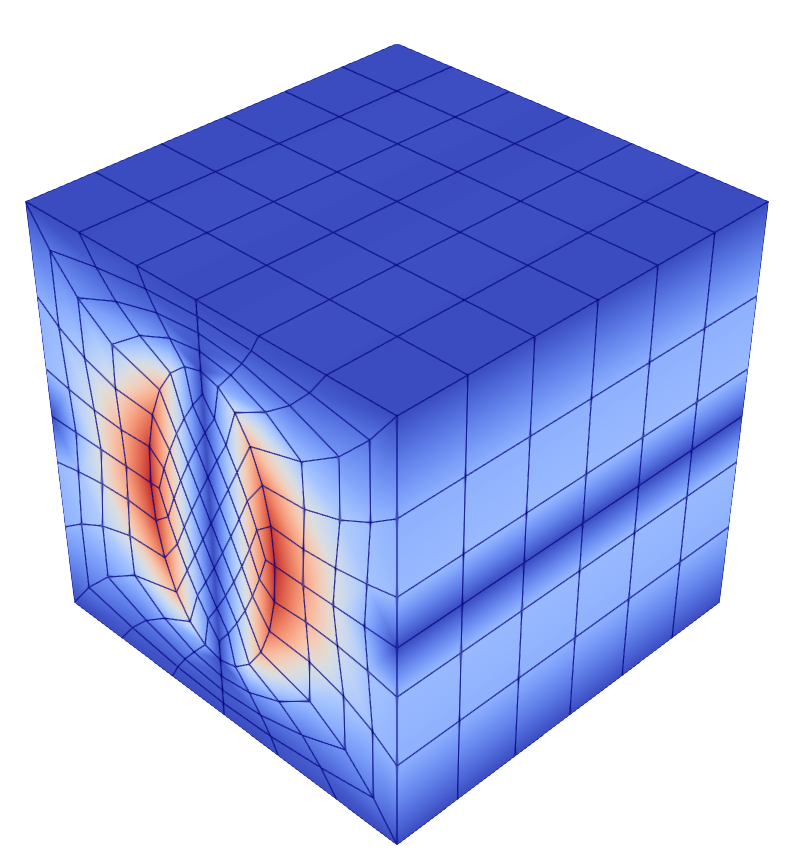
\includegraphics[width=\textwidth]{Figures/xx.png}
        \caption{$\bar{\varepsilon}_{xx}$}
    \end{subfigure}
    \hfill
    \begin{subfigure}[b]{0.26\textwidth}
        \centering
        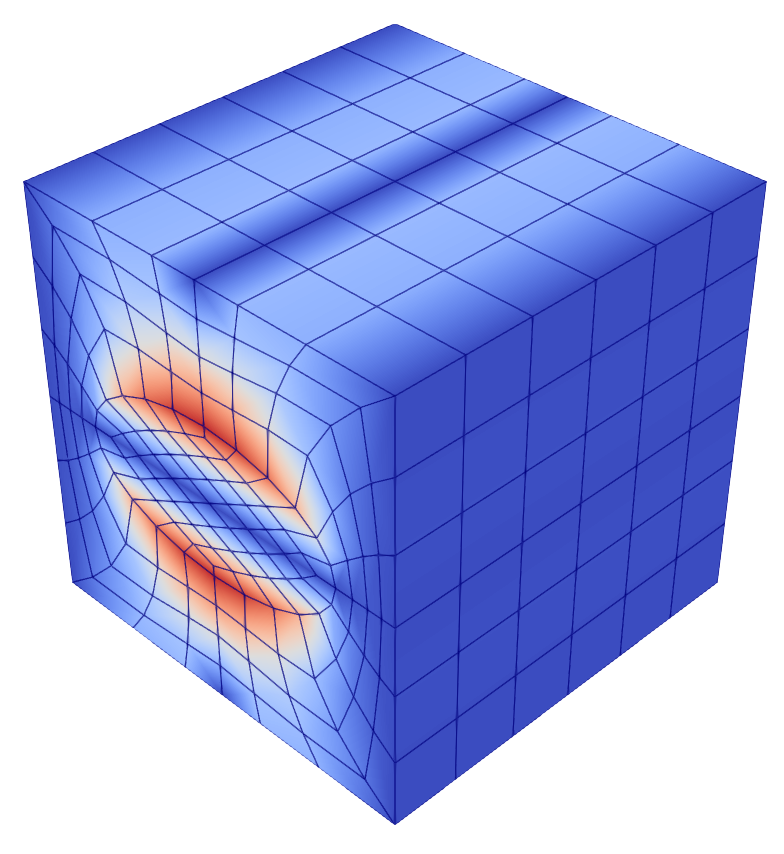
\includegraphics[width=\textwidth]{Figures/yy.png}
        \caption{$\bar{\varepsilon}_{yy}$}
    \end{subfigure}
    \hfill
    \begin{subfigure}[b]{0.34\textwidth}
        \centering
        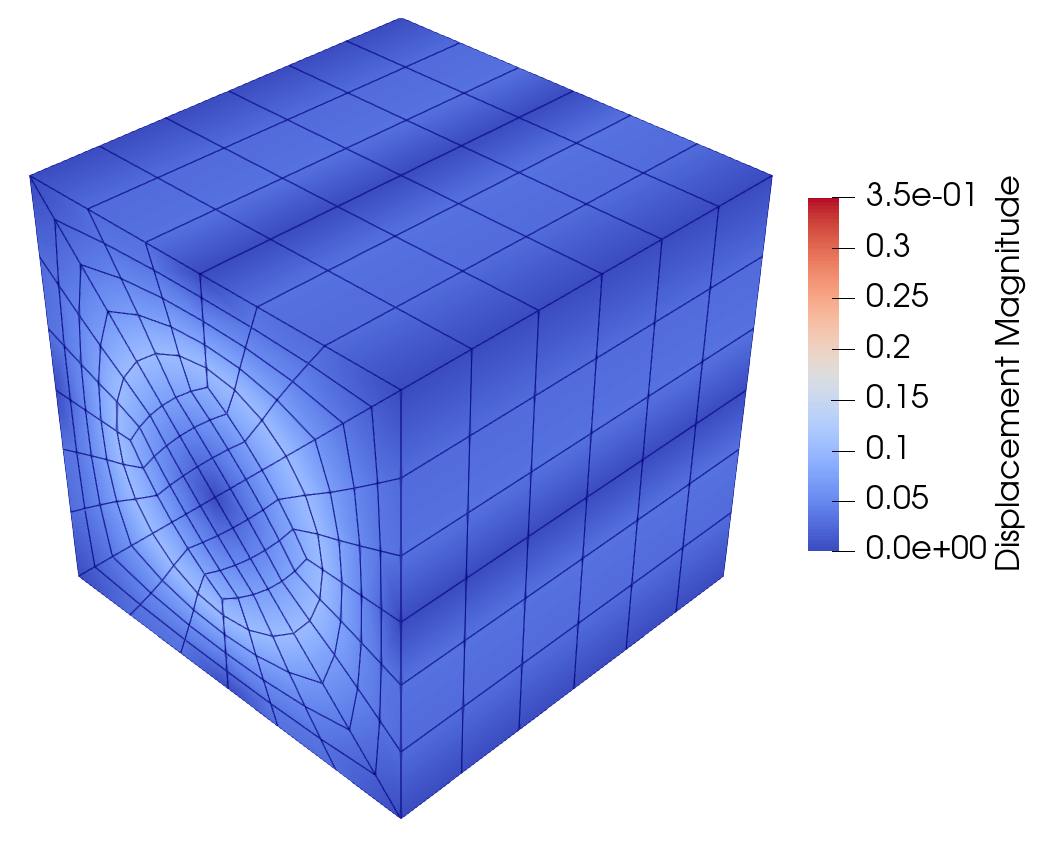
\includegraphics[width=\textwidth]{Figures/zz.png}
        \caption{$\bar{\varepsilon}_{zz}$}
    \end{subfigure}

    \vspace{0.5cm}

    % ---------------- Row 2 ----------------
    \begin{subfigure}[b]{0.26\textwidth}
        \centering
        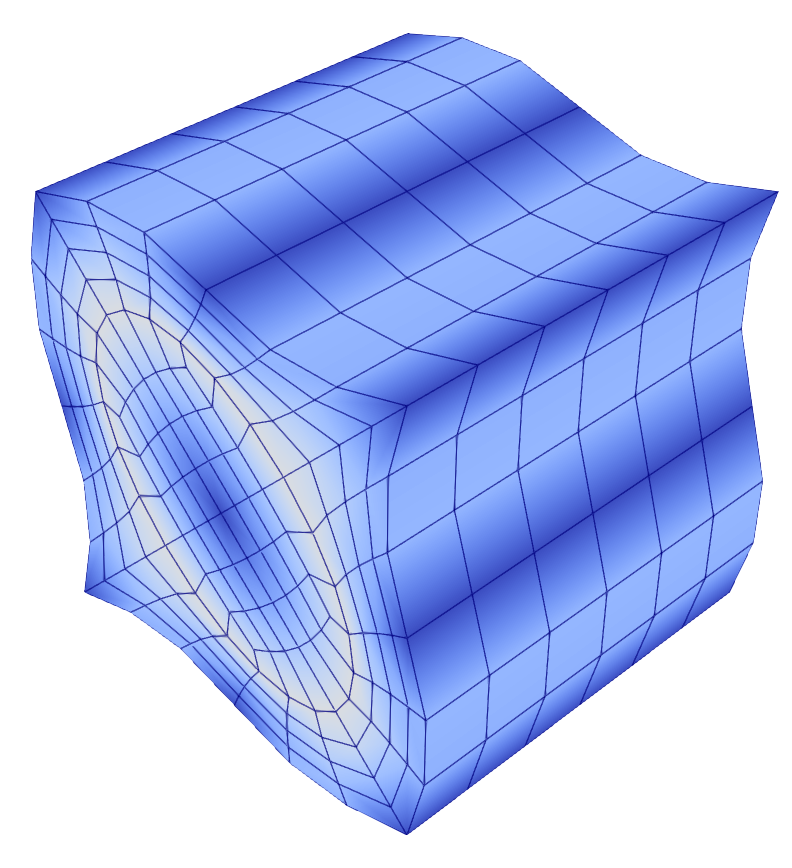
\includegraphics[width=\textwidth]{Figures/xy.png}
        \caption{$\bar{\varepsilon}_{xy}$}
    \end{subfigure}
    \hfill
    \begin{subfigure}[b]{0.26\textwidth}
        \centering
        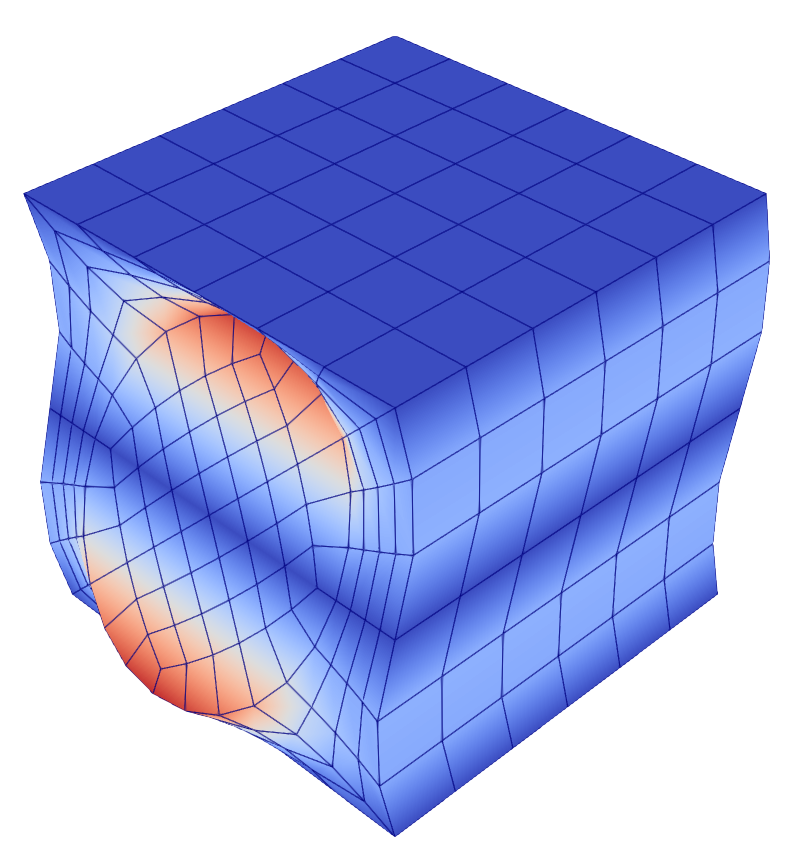
\includegraphics[width=\textwidth]{Figures/yz.png}
        \caption{$\bar{\varepsilon}_{yz}$}
    \end{subfigure}
    \hfill
    \begin{subfigure}[b]{0.26\textwidth}
        \centering
        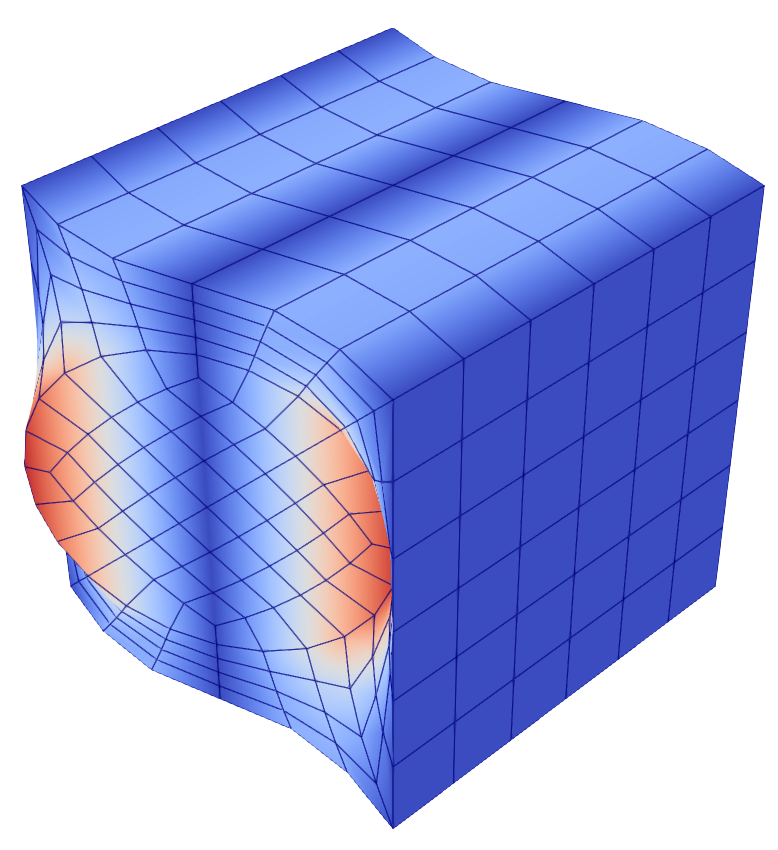
\includegraphics[width=\textwidth]{Figures/xz.png}
        \caption{$\bar{\varepsilon}_{xz}$}
    \end{subfigure}

    \caption{Macroscopic strain influence functions associated with the six independent strain modes used in the EBH offline stage.}
    \label{fig:macro_modes}
\end{figure}


\subsection{Comparison old code (Fortran) and parallelized code (FEniCS)}

\begin{figure}[htbp]
	\centering
	\begin{subfigure}[t]{0.48\textwidth}
		\centering
		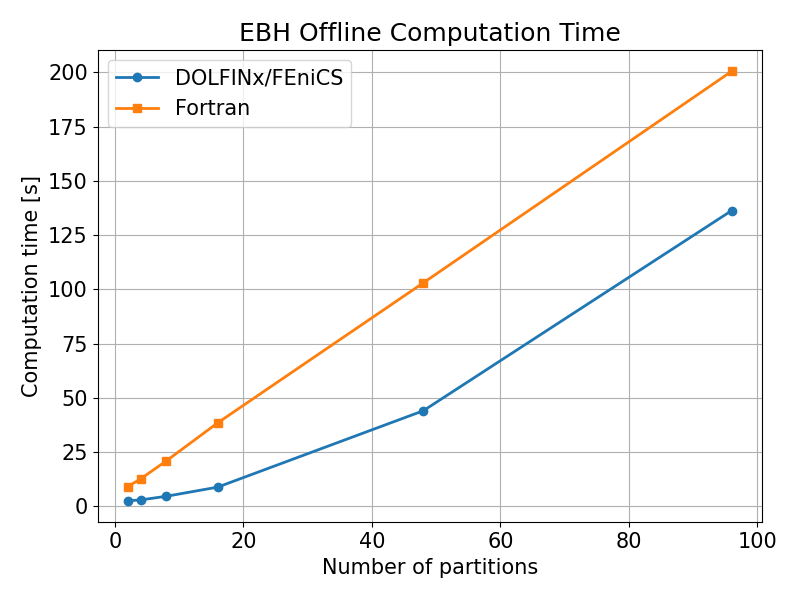
\includegraphics[width=7cm]{Figures/Figure_2.png}
		\caption{Computation time}
		\label{fig:time1}
	\end{subfigure}\hfill
	\begin{subfigure}[t]{0.48\textwidth}
		\centering
		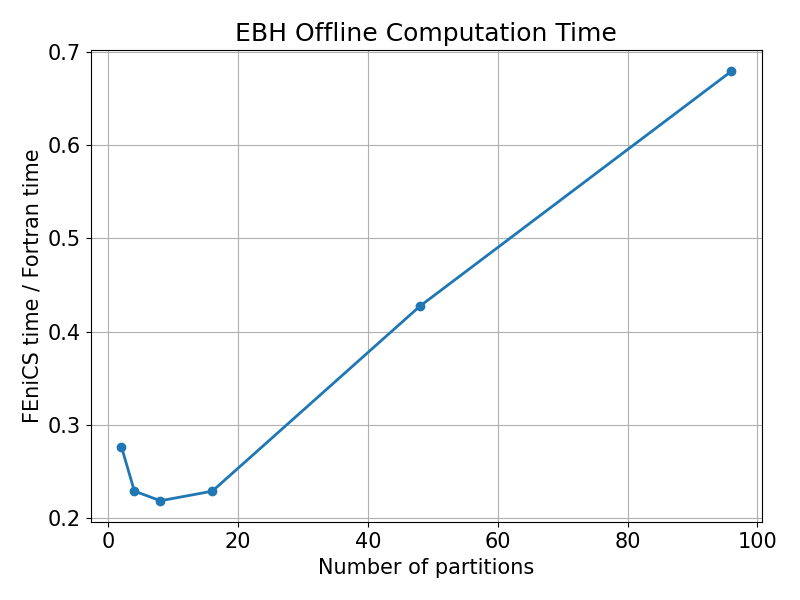
\includegraphics[width=7cm]{Figures/Figure_1.png}
		\caption{Ratio between Python code and Fortran code}
		\label{fig:time2}
	\end{subfigure}
	\caption{Time results}
	\label{fig:}
\end{figure}

Figure~\ref{fig:time1} compares the offline computation time between the original serial Fortran implementation and the proposed parallel DOLFINx implementation for different numbers of EBH partitions, using 8 MPI ranks.

The results show that both implementations exhibit an increasing computational cost as the number of partitions grows. This behavior is expected since the number of influence problems scales as
\begin{equation}
N_{\mathrm{solves}} = 6 + 6N_{\mathrm{part}}
\end{equation}

meaning that each additional partition introduces six additional linear systems associated with the $P$ influence functions.

However, the DOLFINx implementation consistently outperforms the Fortran implementation for all partition counts. For small numbers of partitions, the difference is moderate, while for larger partition counts the advantage becomes significantly more pronounced. For example, at 96 partitions the DOLFINx implementation reduces the total computation time from approximately $200\,\mathrm{s}$ to $136\,\mathrm{s}$.

This improvement is primarily attributed to three factors:

\begin{enumerate}
    \item Reuse of the sparse matrix factorization for multiple right hand sides.
    
    \item Use of the MUMPS sparse direct solver through PETSc, avoiding the dense matrix operations employed in the Fortran implementation.
    
    \item Task level MPI parallelization, where independent EBH influence problems are distributed across MPI ranks.
\end{enumerate}


Figure \ref{fig:time2} shows the ratio between the DOLFINx and Fortran computation times. The ratio remains below one for all cases, confirming that the proposed implementation is consistently faster. For low partition counts, the DOLFINx implementation requires approximately $20\%-30\%$ of the Fortran computational time. As the number of partitions increases, the ratio grows moderately due to the increasing cost of repeated sparse solves and communication overheads, but the parallel implementation still maintains a clear performance advantage.

\subsection{Comparison with paper}
To verify the correctness of the computed influence tensors, the obtained $E$ and $P$ tensors were used in the EBH online stage. The online implementation was provided by one of the authors (Junhe Cui \cite{FishCuiEBH}) of the original EBH work and was used as a reference solution for validation purposes.

Figure \ref{fig:validation} compares the macroscopic stress response obtained in the present implementation against the reference EBH results reported in the original work for the case with 96 matrix partitions. The comparison shows very good agreement for the stress components $\bar{S}_{11}$, $\bar{S}_{22}$, and $\bar{S}_{33}$ under the applied loading path.

The obtained curves reproduce the same nonlinear behavior and stress evolution observed in the reference solution, indicating that the offline influence tensors were correctly assembled and that the partition level RVE computations were successfully integrated into the online EBH formulation.


\begin{figure}[htbp]
    \centering
    \begin{subfigure}[t]{0.48\textwidth}
        \centering
        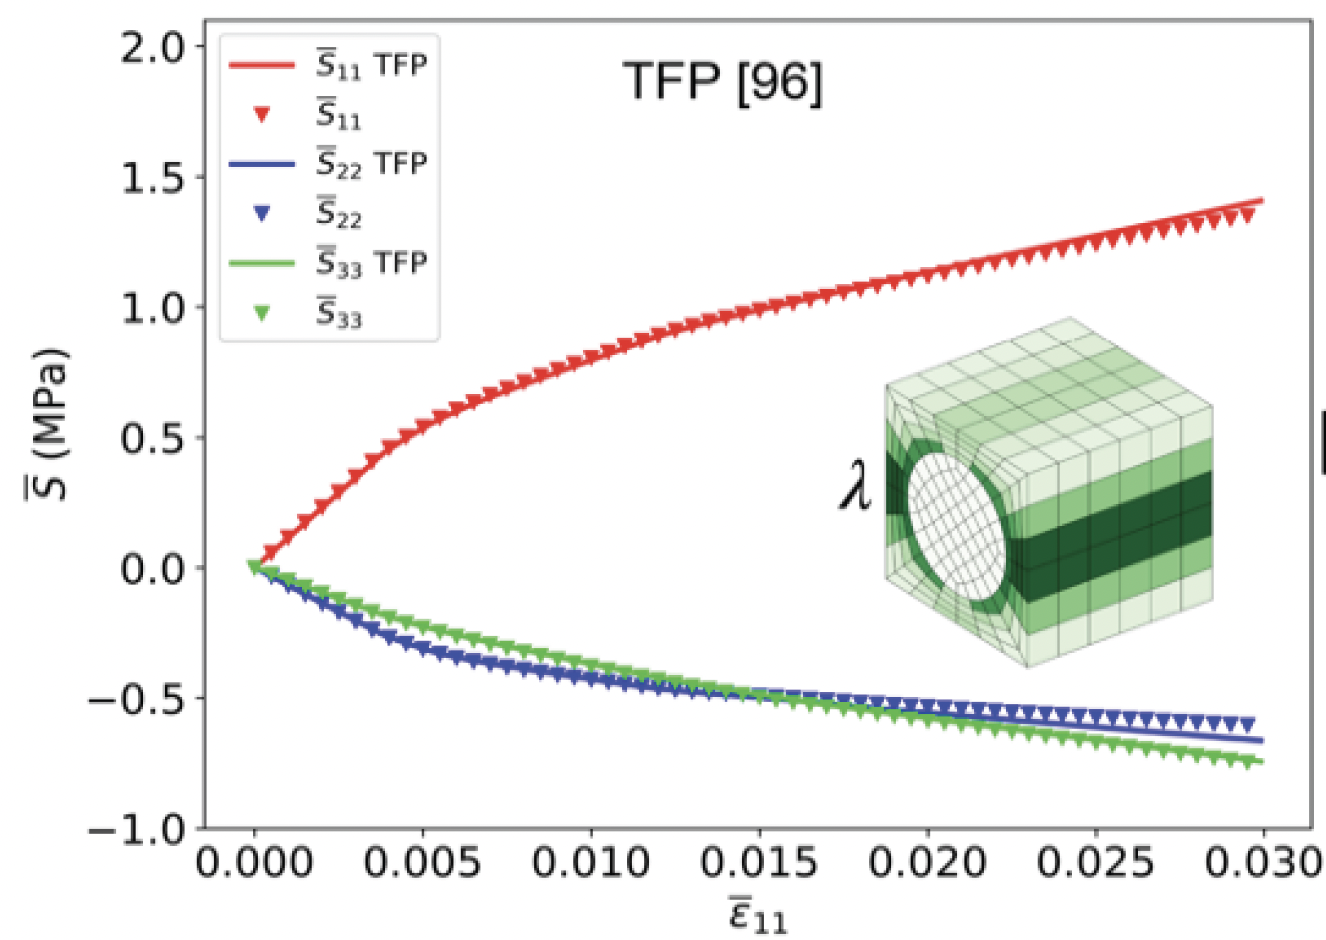
\includegraphics[width=7cm]{Figures/paper.png}
        \caption{EBH paper}
        \label{fig:ebh}
    \end{subfigure}\hfill
    \begin{subfigure}[t]{0.48\textwidth}
        \centering
        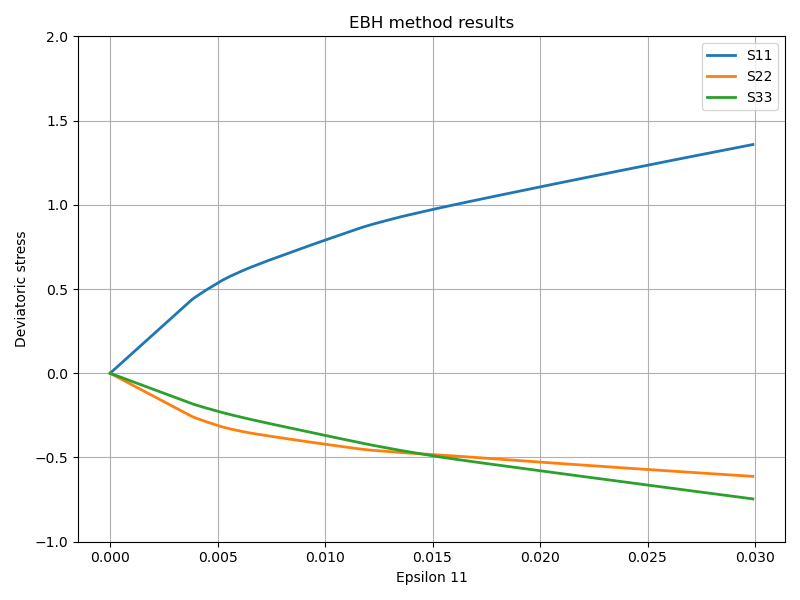
\includegraphics[width=7cm]{Figures/ebh.png}
        \caption{My results}
        \label{fig:}
    \end{subfigure}
    \caption{Validation against paper EBH}
    \label{fig:validation}
\end{figure}

\section{Conclusions}

This project implemented and tested a task parallel strategy for the EBH offline stage. The main goal was to accelerate the computation of the partition level influence tensors $E$ and $P$, which are required by the reduced order EBH formulation for nonlinear multiscale simulations.

The DOLFINx implementation successfully computes the RVE influence functions using periodic boundary conditions enforced through multi point constraints. Since all influence problems share the same stiffness matrix, the matrix was assembled and factorized only once per MPI rank, and then reused for multiple right hand sides. This significantly reduced the cost compared with repeatedly solving each RVE problem independently.

The results show that the proposed DOLFINx implementation is consistently faster than the original serial Fortran implementation for all tested numbers of partitions. The improvement is mainly due to the use of sparse linear algebra through PETSc/MUMPS, reuse of the matrix factorization, and task level MPI parallelization of the independent EBH right hand side problems. As expected, the computational cost increases with the number of partitions because the number of $P$ influence problems scales as $6N_{\mathrm{part}}$.

The computed influence tensors were also verified by using them in the EBH online stage provided by Junhe Cui. The resulting macroscopic stress response showed good agreement with the reference EBH results, indicating that the offline tensors were correctly assembled and that the parallelized computation preserves the expected physical response.

Overall, the project demonstrates that the EBH offline stage is naturally suitable for task parallelization, since the partition level RVE problems are independent. This approach provides a practical way to reduce the offline cost of reduced order homogenization methods, especially when a large number of partitions is required to represent nonlinear localization effects.

\bibliographystyle{plainnat}

\bibliography{references}

\end{document}
